\section{Experiments}%
\label{sec:experiments}

In this section, we will apply the techniques presented in the previous sections
to the Bouncing Ball example introduced in~\cite{Manfred2019}. In that example,
a ball is given by its position and velocity as it bounces up and down from the
floor. A controller is given the choice between two actions --- hit or do
nothing --- and is tasked with keeping the ball bouncing for as long as possible
with as few hits as possible.

We perform the following steps:

\begin{itemize}
    \item Synthesize a strategy in UPPAAL Stratego. This gives us two Q-trees
        (one for $a = 1$ (hit) and one for $a = 0$ (no hit)) with a combined
        number of paths 13,405.
    \item Convert the Q-trees to a single decision tree following the procedure
        described in Section~\ref{sec:convergeToDT}. The conversion is followed
        by simple pruning (Section~\ref{sub:simplePrune}). The resulting tree
        has 84,336 paths and the entailed partitioning can be seen in
        Figure~\ref{fig:ballPartitioningBefore}.
    \item Run the \texttt{MaxPartitions} algorithm on the converted tree. This
        reduces the number of partitions to only 703.
    \item Construct a decision tree to represent the new partitioning as
        described in Section~\ref{sub:regionsToDT}. This gave a tree with 892
        paths. The resulting partitioning is seen in
        Figure~\ref{fig:ballPartitioningAfter}.
    \item Generate samples from 1000 runs with a maximum of 300 time steps each,
        logging the state at every 0.5 time step. This gives 600,000 sample data
        points which we use for empirical pruning, resulting in a tree of just
        189 paths.
    \item \textit{Now maybe something about my analytical pruning that got the
        tree down to just 164 paths}
    \item Export all versions of the strategy to UPPAAL Stratego format and
        compare performance on the system. Results are shown in
        Table~\ref{tab:minimizedResults}.
\end{itemize}

A couple of things are of notable interest here.

First, converting the strategy from a set of Q-trees to a decision tree vastly
increases the total number of paths. Without any minimization effort, it seems
that the decision tree of size 84,336 does not yield any particular advantages
in terms of explainability and interpretability compared to the two Q-trees with
a combined size of 13,405 paths. For cases where there are more variables or
possible actions, this would most likely pose an even greater issue.

\begin{table}[ht]
    \centering
    \caption{%
        Comparing the performance of controllers for the bouncing ball example
        over 1000 runs for 120 time steps each before and after various attempts
        at minimizing the size through either empirical pruning or the
        \texttt{MaxPartitions} algorithm.
    }\label{tab:minimizedResults}
    \begin{tabular}[t]{lccc}
        \toprule
        Version & Paths & Expectation (hits) & Deviation \\
        \midrule
        Q-trees & 13,405 & 38.401 & 0.177 \\
        Original DT & 84,336 & 38.431 & 0.178 \\
        MaxPartitions & 895 & 38.435 & 0.177 \\
        MaxPartitions then Prune & 189 & 38.347 & 0.173 \\
        % MaxPartitions, EmpPrune and AnaPrune & 164 & 38.311 & 0.172 \\
        \bottomrule
    \end{tabular}
\end{table}

Second, the effect of \texttt{MaxPartitions} is a drastic reduction in the
number of partitions. Even though the list of regions cannot be perfectly
represented by a decision tree and the number of paths in the constructed tree
thus increases a bit, the tree of size 892 is a decisive improvement from both
the original set of Q-trees and the especially the converted tree.

Third, the decreasement in the number of paths after empirically pruning the
tree indicates that many areas of the state space are never visited in practice.
It is also remarkable, that by utilizing this sample data we can further reduce
the already minimized tree by a factor of 4 without sacrificing performance.

\begin{figure}[ht]
    \begin{subfigure}[b]{.4\textwidth}
        \centering
        \includegraphics[width=0.8\textwidth]{ballPartitioningBefore}
        \subcaption{%
            Original paritioning
        }\label{fig:ballPartitioningBefore}
    \end{subfigure}
    \begin{subfigure}[b]{.4\textwidth}
        \centering
        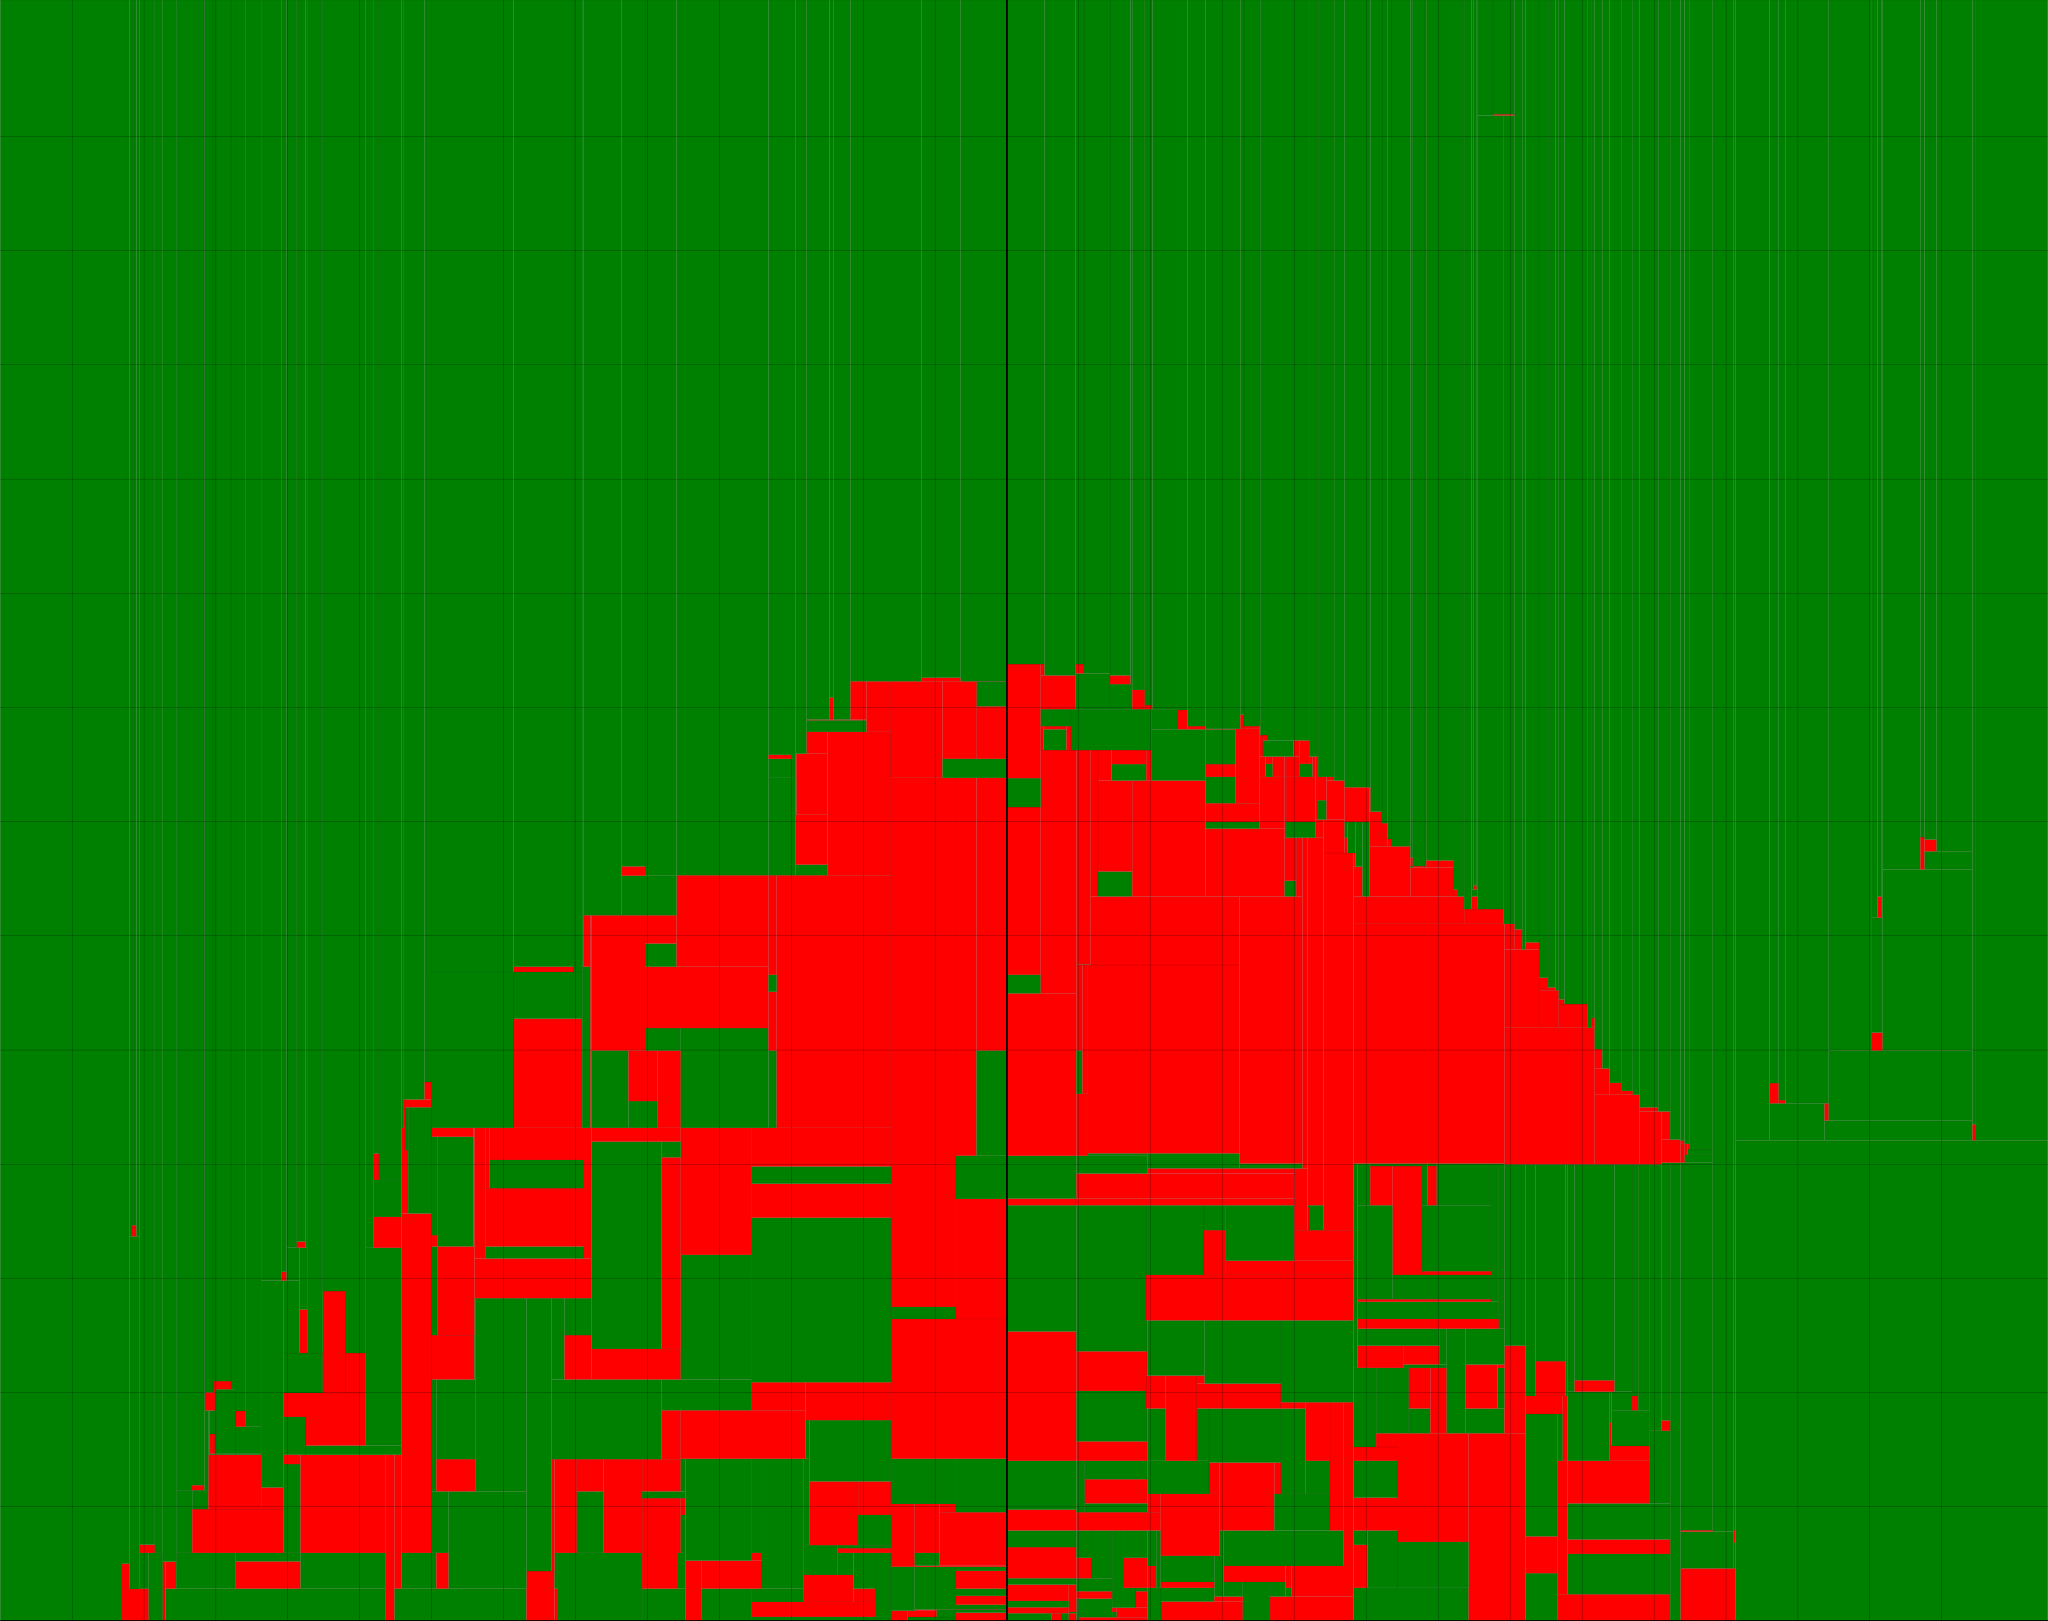
\includegraphics[width=0.8\textwidth]{ballPartitioningAfter}
        \subcaption{%
            Partitioning after \texttt{MaxPartitions}.
        }\label{fig:ballPartitioningAfter}
    \end{subfigure}
    \caption{%
        A 2D visualization of the partitioning (dotted lines) of the state space
        before and after \texttt{MaxPartitions}. The x-axis is velocity and the
        y-axis is the balls position. Green areas represents the action `no
        hit', red areas represents `hit'.
    }\label{fig:ballPartitioning}
\end{figure}

\subsection{dtControl}%
\label{subsec:dtControl}\todo{This is very experimental}

The tool \texttt{dtControl}~\cite{dtControl2} has the ability to take a
synthesized strategy represented as a look-up table and convert the
representation to a decision tree that respects the safety requirements but
compresses the size immensely.  This is naturally of great interest for our
case, but both the Q-tree representation and our own decision tree conversion
alters the setup somewhat.

However, even though the tool actually supports directly working with the output
format of UPPAAL Stratego, this is only the case for strategies learned using
the \texttt{control[]} directive, which controls for certain defined safety
parameters to always be respected. In our case of the bouncing ball example, the
controller is trained with the \texttt{minE[]} directive, which minimizes a
given parameter (in this case, the number of times the controller hits the
ball).

Instead, we had to create our own output files to use as input for
\texttt{dtControl}. According to the documentation, a controller strategy can be
specified in a simple CSV format where each line contains an allowed
state/action pair, that is, $N$ values representing a state where the following
$M$ values constitutes an allowed action. For example, in the case of the
bouncing ball, we have two state variables (position and velocity) and one action
variable (hit or not hit), meaning each line would have three values.

We have attempted two experiments with different ways of specifying our original
controller.

In the first experiment, we used the trained controller to generate 30,000
samples of state/action pairs. That is, the UPPAAL model was run for 300
time steps with the trained controller deciding what action to take in each
encountered state and then the state/action pairs were logged at each 0.01
time step.

In the second experiment, we converted the strategy a set of Q-trees (the
initial UPPAAL format) to a DT as described in Section~\ref{sec:convergeToDT}.
This DT had a partition size (number of leaves/paths) of 91,054. We used these
partitions as the input data to \texttt{dtControl} by taking the maximum value
of each variable in each individual partition together with the optimal action
of that state. That is, we effectively specified the discretization of the state
space by defining the bounds of each state paired with the allowed/optimal
action.

\begin{table}[ht]
    \centering
    \caption{%
        Comparing the performance of controllers for the bouncing ball example
        over 1000 runs for 120 time steps each before and after various attempts
        at minimizing the size through \texttt{dtControl}.  
    }\label{tab:dtcontrolTable}
    \begin{tabular}[t]{lccc}
        \toprule
        Version & Paths & Construction time & Expectation (hits) \\
        \midrule
        Original DT & 91,054 & --- & 38.431 \\
        Samples & 27,234 & 8:14 & 318.411 \\
        State bounds & 521 & 0:41 & 315.769 \\
        \bottomrule
    \end{tabular}
\end{table}


The results when applying the generated strategies to the model in UPPAAL are
given in Table~\ref{tab:dtcontrolTable} together with the baseline original
decision tree directly converted from the Q-tree set. As is seen, when we used
samples, we still got a somewhat large DT that took more than 8 minutes to
generate. And the performance (expected number of hits) is substantially worse
than the baseline version. For the version based on state bounds, we got a much
smaller tree with only 521 paths, but the performance was still very far from
the original.


